\documentclass[12pt, a4paper, openright, draft]{memoir}
\usepackage{fontspec}
\let\ordinal\relax %! Fixes \ordinal conflict with memoir
\usepackage[us]{datetime}
\newdate{startdate}{15}{3}{2020}
\usepackage{paracol}

\usepackage{expex, tikzvowel, phonrule}


\usetikzlibrary{fit}
\newdimen\contourraise
\newdimen\contourspacetokenwidth
\newcount\lasttokennumber
\newcount\currenttokennumber
\newcount\contourmarkcount
\newcount\contourtokenunderlinestate
\newbox\contourbox

\tikzset{
  tight fit/.style={
      inner sep=0pt,
      outer sep=0pt,
    },
  %
  %
  % How far above the reference anchor of the text,
  contour raise/.code=\pgfmathsetlength\contourraise{#1},
  contour reference anchor/.store in=\contourreferenceanchor,
  contour reference anchor=base east,
  % The `scale' for the values in the contour height specification
  contour scale/.store in=\contourscale,
  contour scale=3pt,
  % The prefix for the contour marks.
  contour mark prefix/.store in=\contourmarkprefix,
  contour mark prefix=contour,
  % The style for the contour path
  contour/.style={
      draw,
      rounded corners=1ex,
    },
  % The style for the token nodes
  every contour token/.style={
      anchor=base west,
      inner sep=0pt,
    },
  contour underline/.style={
      draw
    },
  % The character to insert a mark (use with care)
  contour mark character/.store in=\contourmarkchar,
  contour mark character=|,
  % Want to change the code for contour marks? Use this key.
  contour mark code/.store in=\contourmarkcode,
  % Want to change the code for tokens? Use this key.
  contour token code/.store in=\contourtokencode,
  % Want to change the code for drawing the contour? Use this  key.
  contour code/.store in=\contourcode,
  %
  % Default stuff
  contour mark code={%
      \coordinate (\contourmarkprefix-\the\contourmarkcount)
      at ([yshift=\contourraise, y=\contourscale,
        shift={(0,\currentcontourheight)}]token-\the\currenttokennumber.\contourreferenceanchor);
    },
  contour token code={%
      \node [every contour token/.try] at
      (token-\the\lasttokennumber.base east)
      (token-\the\currenttokennumber) {\token};
    },
  contour code={
      \draw [contour] (\contourmarkprefix-1)
      \foreach \y in {2,...,\the\contourmarkcount}{ --
          (\contourmarkprefix-\y) };
    },
  %
  % Don't draw the contour.
  tokens only/.style={
      contour code={}
    },
  %
  % Only draw the contour (but the space is still used for the tokens)
  contour only/.style={
      every contour token/.append style={
          execute at begin node={\setbox\contourbox=\hbox\bgroup},
          execute at end node=\egroup\phantom{\box\contourbox}%
        },
      underline/.style={
          draw=none
        }
    },
  %
  % Make tokens follow the contour marks.
  tokens follow contour/.style={
      tokens only,
      contour token code={%
          \node [every contour token/.try, y=\contourscale] at
          (token-\the\lasttokennumber.base east |-
          0,\currentcontourheight)
          (token-\the\currenttokennumber) {\token};
        },
    },
  % What style to use when drawing underline
  underline/.style={
      draw
    },
  % The underline is drawn along the south side of a node which
  % takes this style.
  underline token/.style={
      inner ysep=1pt
    },
  % When grouping tokens (e.g., for putting box around)
  % this style is applied to a node that is fitted around the group
  token group/.style={
      inner xsep=1pt,
      inner ysep=2pt,
      rounded corners=2pt
    },
  % Draw boxes around tokens groups.
  box tokens/.style={
      token group/.append style={
          draw
        }
    },
  % Change the width of the spaces.
  space token width/.code=\pgfmathsetlength\contourspacetokenwidth{#1},
  space token width=0.125cm
}

\makeatletter

\def\at@{@}

\newcommand\contour[2][]{%
  \begin{scope}[#1]
    \coordinate (token-0);
    \currenttokennumber=0\relax%
    \lasttokennumber=0\relax%
    \contourmarkcount=0\relax%
    \def\lastcontourheight{0}%
    \contourtokenunderlinestate=0\relax%
    \@contour#2@%
    }

    % Must check for a spaces
    \def\@contour{\futurelet\@token\@checkforspace}

    \def\@uscore{_}
    \def\@checkforspace{%
      \ifx\@token\@sptoken%
        \let\@next=\@replacespace%
      \else%
        \if\@token\contourmarkchar%
          \let\@next=\@contour@insertmark
        \else%
          \if\@token\@uscore
            \let\@next=\@contourtoggleunderline%
          \else%
            \let\@next=\@@contour%
          \fi%
        \fi%
      \fi%
      \@next%
    }

    \def\@contourtoggleunderline#1{%
      \advance\contourtokenunderlinestate by1\relax
      \ifnum\contourtokenunderlinestate>3\relax%
        \contourtokenunderlinestate=0\relax%
      \fi%
      \@contour%
    }

    \def\@contour@insertmark{%
      \afterassignment\@@contour@insertmark\let\@token=%
    }

    \def\@@contour@insertmark{%
      \futurelet\@token\@@@contour@insertmark}%

    \def\@@@contour@insertmark{%
    \if\@token[%
      \let\@next=\@@@@contour@insertmark%
    \else%
      \let\currentcontourheight=\lastcontourheight%
      \let\@next=\@@@@@contour@insertmark%
    \fi%
    \@next%
    }

    \def\@@@@contour@insertmark[#1]{%
      \def\@tmp{#1}%
      \ifx\@tmp\@empty%
        \let\currentcontourheight=\lastcontourheight%
      \else%
        \def\currentcontourheight{#1}%
      \fi%
      \@@@@@contour@insertmark}

    \def\@@@@@contour@insertmark{%
      \advance\contourmarkcount by1\relax%
      % Code for inserting mark
      \contourmarkcode%
      \let\lastcontourheight=\currentcontourheight%
      \@contour}

    \def\contourspacetoken{{\hbox to \contourspacetokenwidth{\hfill}}}

    \def\@replacespace#1{%
      \@contour\contourspacetoken#1%
    }

    \def\@@contour#1{%
      \def\@token{#1}%
      \if\@token\at@%
        \@contourdounderline%
        \pgfutil@ifundefined{pgf@sh@ns@tokengroup}{}{%
          \node [tight fit, fit={(tokengroup)}, token group/.try] {};
          \global\let\pgf@sh@ns@tokengroup=\relax%
        }%
        \let\@next=\@@@contour%
      \else%
        \lasttokennumber=\currenttokennumber%
        \advance\currenttokennumber by1%
        \let\token=\@token%
        % Code for typesetting token
        \contourtokencode%
        % Manage underline state
        \@contourdounderline%
        \def\@@token{\contourspacetoken}%
        \ifx\@token\@@token%
          \pgfutil@ifundefined{pgf@sh@ns@tokengroup}{}{%
            \pgfutil@ifundefined{pgf@sh@ns@underline}{}{%
              \node [tight fit, fit={(tokengroup) (underline)}]
              (tokengroup)
              {};}%
            \node [tight fit, fit={(tokengroup)}, token group/.try] {};
            \global\let\pgf@sh@ns@tokengroup=\relax%
          }%
        \else
          \pgfutil@ifundefined{pgf@sh@ns@tokengroup}{%
            \node [tight fit,
              fit={(token-\the\currenttokennumber)}]
            (tokengroup) {};
          }{%
            \node [tight fit,
              fit={(token-\the\currenttokennumber)
                  (tokengroup)}]
            (tokengroup){};
          }%
        \fi%
        \let\@next=\@contour
        %
      \fi%
      \@next%
    }

    \def\@contourdounderline{%
      \ifcase\contourtokenunderlinestate%
      \or
        \node [tight fit, fit={(token-\the\currenttokennumber)}]
        (underline) {};
        \contourtokenunderlinestate=2\relax%
      \or%
        \node [tight fit,fit={(token-\the\currenttokennumber) (underline)}]
        (underline) {};
      \or%
        \node [tight fit, fit={(underline)}, underline token/.try]
        (underline) {};
        \draw [underline/.try]
        (underline.south west) -- (underline.south east);
        \pgfutil@ifundefined{pgf@sh@ns@tokengroup}{}{%
          \node [tight fit, fit={(tokengroup) (underline)}]
          (tokengroup) {};%
          \node [tight fit, fit={(tokengroup)}, token group/.try] {};
          \global\let\pgf@sh@ns@tokengroup=\relax%
          \global\let\pgf@sh@ns@underline=\relax%
        }
        \contourtokenunderlinestate=0\relax
      \fi%
    }
    \def\@@@contour{%
    \ifnum\contourmarkcount>1
      % Code for drawing contour
      \contourcode%
    \fi%
  \end{scope}%
}

\makeatother


\usepackage[hidelinks]{hyperref}
\hypersetup{linktoc=all}

\titlingpageend{\clearforchapter}{\clearforchapter} %! Titlingpage/openany fix for blank page
\pagestyle{ruled}
\makeoddfoot{plain}{}{}{\thepage}
\makeevenfoot{plain}{\thepage}{}{}
\copypagestyle{title}{empty}

\setmainfont{Libertinus Serif}

\setlength{\parindent}{0pt}
\nonzeroparskip

\lingset{
  glstyle=nlevel,
  belowglpreambleskip={-.5\parskip},
  aboveglftskip={-.5\parskip},
  exskip={0pt},
  glneveryline={,\it,\nogloss}
}

% Doc specific stuff
\newcommand{\langword}[1]{\textit{#1}}
\newcommand{\langname}{Ahale}

\newcommand{\pronounced}[1]{\vskip-0.5\parskip[#1]}


\begin{document}
\title{\langname : A Complete Reference}
\author{Pancake}
\date{\DTMusedate{startdate} -- \DTMtoday}
\frontmatter
\begin{titlingpage}
  \maketitle
\end{titlingpage}

\begin{KeepFromToc}
  \tableofcontents
\end{KeepFromToc}
\mainmatter

\chapter{Introduction}\label{ch:introduction}
\section{Conventions}\label{sec:conventions}
In this document, italic text will be used for native \langname\ words, unless enclosed in angle brackets (\nativetext{ahale} or \orthotext{ahale}, but never \orthotext{\nativetext{ahale}}).
\aside{This aside is from an internal perspective. It may discuss things such as word choice, or the cultural significance of phrases.}
\aside{\fleuron\ This aside is from an external perspective. It may discuss design choices or other such self-imposed challenges.}
The former is found mostly in running prose, and the latter in places where a word is being used as a more self-contained example, or simply if orthography is of particular interest.

\phomtext{forward slashes} are used for phonemic transcriptions, while \phontext{square brackets} are used for phonetic transcriptions.

When words are exemplified within prose, they are often followed by a short translation. These will be written surrounded by \transtext{single quotes}.

Notable terms will be written \notabletext{like this.}

``Double quotes'' are used for non-standard, ironic, or otherwise deviant use of terms.

\subsection{Document Structure}
Most of the content contained within this grammar will be found in the main prose. However, footnotes along with margin notes will be used for tangential or, in the case of footnotes, explanatory details about particular terms.

Margin notes will be reserved for explanation of decisions made in the various translations, or in the usage details of a specific construction.
In the case of notes from an external perspective, being preceded by a fleuron (\fleuron).

\subsection{Glossing}\label{sec:conventions-gloss}
Glosses are generally constructed as follows:

\begin{example}
  \lect Dialect
  \preamble Romanization (undelimited)
  \pronunciation pronunciation
  \gloss
    morphemic & morphemic \\
    transcription & transcription \\
    (object language) & (metalanguage) \\
  \tr Translation
  \source Source
\end{example}

\section{History}\label{sec:history}
\subsection{Internal}\label{sec:hist-int}

\subsection{External}\label{sec:hist-ext}
\langname\ is the spiritual successor to my first conlang, Wei. As with many first attempts at conlanging, I consider Wei to be poorly made, and even more poorly described. Because of this, I consider \langname\ a successor only on account of my initial intentions.

Wei was very anglocentric, only a few steps away from a full relex, if even that. After I pronounced Wei abandoned in September 2019, I took a long break, and used that time to learn more about linguistics so that when I returned, I felt at least somewhat more prepared to make something I would be proud of.

When I began work on \langname , I wanted to stray as far away from my original mistakes as I could do comfortably. With that in mind, I outlined just a few goals for myself:

\begin{itemize}
  \item A morphosyntactic alignment other than nominative-accusative
  \item A minimalistic phonology which I would still be comfortable pronouncing
  \item Relatively free word order
  \item Some degree of non-concatenative morphology
  \item Thorough documentation, with many examples to explain nuances in translation (another goal of mine)
  \item Generally be interesting, fun, and fulfilling to work on
\end{itemize}

As the documentation currently stands, I feel I have achieved, and continue to work to achieve many of these goals. Depth of documentation, and nuance of lexical entries is something I'm still working on. Throughout the various iterations of this document, I hope that I can continue to improve on these areas to an even greater extent than I have at the time of writing this section.\footnotemark

\footnotetext{Last updated \DTMdisplaydate{2021}{1}{31}{-1}
}
\subsubsection{Typological Details}
While I don't find typology a terribly informative tool in regards to how language \textit{actually} functions, it can serve as an overview of concepts which will be encountered. As such, here's (another) short list of bullet points:

\begin{itemize}
  \item Utilizing a direct-inverse verbal system (resulting in a syntactically \textit{hierarchical} alignment)
  \item Ergative-absolutive morphology
  \item Strong pro-drop tendencies
  \item (A lot of) reduplication
  \item Use of verb serialization
\end{itemize}

In essence, the things which I find interesting.

\part{Phonology}\label{prt:phonology}
\chapter{Segmental Phonology}\label{ch:seg-phono}
\section{Inventory}\label{sec:phono-inv}

\begin{table}[ht]
  \centering
  \begin{tabular}{*{7}{c}}
    \toprule
    & Labial & Alveolar & Velar & Glottal \\\midrule
    Plosive   & p      & t        & k     & ʔ       \\
    Nasal     & m      & n        &       &         \\
    Fricative & ɸ      & s        & x     & h       \\
    Sonorant  & w      & l        &       &         \\
    \bottomrule
  \end{tabular}
  \caption{Consonant Inventory}
  \label{table:consonants}
\end{table}

\aside{\fleuron \phontext{e} is an allophone of \phomtext{ə}, rather than a phoneme unto itself as it may first appear, (see \textsc{rel} and \textsc{assoc} \nativetext{ʔe})
}

\begin{figure}[ht]
  \centering
  \begin{vowel}
    \vpoint{0}{0}{i}
    \vpoint{0}{2}{u}
    \vpoint{1.5}{1}{ə}
    \vpoint{3}{1}{a}
    \varrow{a}{u}
    \varrow{a}{i}
  \end{vowel}
  \caption{Phonemic Vowel Inventory}
  \label{table:vowel_phonemes}
\end{figure}

Diphthongs consisting of \phomtext{ə} + high vowel can be observed in a few words, however these diphthongs are prone to collapse. In all but the most conservative of dialects, these are realized as \phomtext{əi əu} \phontext{e o}.

\vfill %! This is not smart don't do this
\section{Stress}
\subsection{Assignment}
Stress is generally assigned to the initial syllable of a root. However, \phomtext{ə} generally will not recieve stress at this stage and move to the second syllable (even if this is also a schwa).

A subset of affixes (including, but not limited to those which utilize reduplication) are considered ``weak'', in that, like schwa, they repel stress.

Such morphemes will be marked with a comma in morphemic transcription, rather than the usual period used at syllable boundaries. Thus \morphtext{ʔə,} refers to a morpheme \phomtext{ʔə} which repels stress.

\subsection{Realization}
Under most circumstances, lexical stress is realized as a slight rise in pitch on the affected syllable, which then gradually falls back to ``standard'' pitch across the remaining part of the word. Because stress is very strongly initial, this means that generally, pitch will fall gradually across words and phrases.

This is of course also affected by phrase- and sentence-level prosody, which will be discussed in \Cref{ch:suprasegmental-phonology}.

\section{Allophony}
This section will be structured a bit differently from the others encountered thus far. Because allophony and diachronic processes in general occur in a particular order, Sectioning will be used to separate larger processes from those more easily described in standard notation.

While this document will cover some dialectical differences, examples given which include phonetic information Will be in reference to a standard dialect, \textbf{Literary Standard \langname}, Which will be abbreviated LSA

The ordering of rules will begin below, and these larger processes will be contained within subsections which will be referenced in the list.

\begin{enumerate}
  \item {
    Stressed \phomtext{ə} becomes \phontext{e}

    \phon{ə\phonfeat{+stress}}{e}
    }
  \item \titleref{sec:allophony-lengthening}
  \item {
    \phontext{ə} is elided between homorganic consonants

    \phonc{ə}{Ø}{\phonfeat{αcplace} \phold \phonfeat{αcplace}}
    }
    \item {
      \phontext{n} + plosive clusters cause place assimilation of the nasal

      \phonc{\phonfeat{+nasal}}{\phonfeat{αcplace}}{\phold \phonfeat{-cont}}
  }
    \item {
      Nasal + plosive clusters assimilate

      \phonc{\phonfeat{-cont}}{\phonfeat{+nasal}}{\phonfeat{+nasal} \phold}
  }

  \item {
      Unstressed final vowels are elided

      \phonc{V\phonfeat{-stress}}{Ø}{\phold \$}
  }
  % \aside{\fleuron\ If I'm being completely honest, I have no idea why the process of affrication is done with +delayed release. I'm simply following the conventions as outlined by \url{http://www.artoflanguageinvention.com/papers/features.pdf}}
  % \item {
  %     Word final geminated plosives are affricated

  %     \phonc{C\phonfeat{-cont \\ +long}}{C\phonfeat{+del release\footnotemark \\ -long}}{\phold \$}
  % }

\end{enumerate}

\subsection{Prosodic Lengthening}\label{sec:allophony-lengthening}
In some situations, syllable shape can cause gemination of the surrounding syllables--- prosodic lengthening, if you will, to allow for more consistent syllable-timing. The most notable of these situations is when a CV syllable, where C is a plosive, comes after a CVV sequence\footnotemark\ beginning in a non-plosive consonant.

\footnotetext{This is described as a CVV \textit{sequence} rather than a CVV syllable, because this process is not dependent on \phontext{VV} being a true diphthong. This can be seen in the first example, where \phontext{ua} Is not a diphthong but still triggers this change.}

Thus, pairs such as the following hypothetical forms may emerge:
\begin{itemize}
  \item \phomtext{suaki} \phontext{ˈsu.a.kːi} and \phomtext{suki} \phontext{ˈsu.ki}
  \item \phomtext{maipi} \phontext{ˈmai.pːi} and \phomtext{mapi} \phontext{ˈma.pi}
  \item \phomtext{iwəiku} \phontext{ˈi.we.kːu}\footnotemark\ and \phomtext{iwəku} \phontext{ˈi.wə.ku}
\end{itemize}

\footnotetext{This more aggressive simplification of diphthongs may give the appearance that plosives may geminate without an apparent trigger. Of course, this only applies to dialects which do not preserve the original diphthongs.}

\aside{\fleuron\ While moraic analysis of this process is not typical, one might suppose that this process is triggered by a heavy syllable followed by a light one, and that CVV is heavy, while VV is not.}
One thing of note is that the onset of the CVV syllable is mandatory to trigger this process. Observe the following hypothetical forms, Which do not undergo this change due to their VVCV shape:
\begin{itemize}
  \item \phomtext{auku} \phontext{ˈau.ku}
  \item \phomtext{aiʔi} \phontext{ˈai.ʔi}
  \item \phomtext{euti} \phontext{ˈo.ti}
\end{itemize}


% \chapter{Suprasegmental Phonology}\label{ch:suprasegmental-phonology}
On

\part{Morphology}
\chapter{Nominal}\label{ch:morpho-nom}
\section{Inflectional Morphology}\label{sec:morpho-nom-inf}
Inflectional morphology is very limited for nouns. The most marked nouns only inflect for case marking and plurality. However, depending on the context, plurality is optional. Depending on the constructions used, inflection of the noun may be even ungrammatical, where in other situations the same inflection would be entirely sensible.

\subsection{Case Marking}\label{sec:case-marking}
\langname 's case system is incredibly small. it consists solely of the cases used for morphosyntactic purposes; the ergative and absolutive cases. The ergative case is marked with reduplication of the initial syllable, while the absolutive case remains unmarked. This becomes slightly less transparent when this interacts with phonotactics, and when this reduplication triggers allophony.

\aside{\fleuron\ While phonological form is not the main focus of this section, the variation that can occur is such that I find it useful. It \textit{is} true that much of the prose simply reiterates what is found in the pronunciation information found in the gloss, however I consider this approach more useful for grasping the reasoning and triggers behind these phonological changes.}

With \notabletext{CV-initial forms,} this is quite straightforward:

\begin{subexamples}
  \baarucols{2}
  \ex
    \preamble pane
    \pronunciation ˈpa.nə
    \gloss
      pane & person[ABS] \\
  \ex
    \preamble papane
    \pronunciation pa.ˈpa.nə
    \gloss
      pa\allo pane & ERG\allo person \\
\end{subexamples}

\notabletext{V-initial forms} are slightly different, as adjacent vowels cannot be identical. An epenthetic \phomtext{ʔ} is inserted to avoid this.

\begin{subexamples}
  \baarucols{2}
  \ex
    \preamble ana
    \pronunciation ˈa.na
    \gloss
      ana & eye[ABS] \\
  \ex
    \preamble a'ana
    \pronunciation aʔ.ˈa.na
    \gloss
      aʔ\allo ana & ERG\allo eye \\
\end{subexamples}

\begin{subexamples}
  \baarucols{2}
  \ex
    \preamble ele
    \pronunciation ə.ˈle
    \gloss
      ele & heaven[ABS] \\
  \ex
    \preamble e'ele
    \pronunciation əʔ.ə.ˈle
    \gloss
      eʔ\allo ele & ERG\allo heaven \\
\end{subexamples}

\phomtext{ə} initial forms (such as the one above) are particularly interesting, in that they most clearly show an interaction between this process of reduplication and allophony. This reduplication can be described with the morpheme \morphtext{V,}. As a result \phomtext{əʔ.ə.lə} is phonetically \phontext{əʔ.ə.ˈle}, rather than \phontext{əʔ.ˈe.lə} as it would be with a standard morpheme.

\notabletext{CVV-initial forms} undergo a slightly different process. The reduplication in this situation does not even apply to the entire syllable, but rather only to the CV segment.

\begin{subexamples}
  \baarucols{2}
  \ex
    \preamble keuha
    \pronunciation ˈko.ha
    \gloss
      keuha & leaf[ABS] \\
  \ex
    \preamble kekeuha
    \pronunciation kə.ˈko.ha
    \gloss
      ke\allo keuha & ERG\allo leaf \\
\end{subexamples}

Consequently for LSA, the reduplicated vowel may be different than its phonetic realization in the stem due to an underlying diphthong.

\notabletext{VV-initial forms} work similarly to CVV forms, with the addition of an epenthetic \phomtext{ʔ} at the morpheme boundary:

\begin{subexamples}
  \baarucols{2}
  \ex
    \preamble auna
    \pronunciation ˈau.na
    \gloss
      auna & moon[ABS] \\
  \ex
    \preamble a'auna
    \pronunciation aʔ.ˈo.na
    \gloss
      aʔ\allo auna & ERG\allo moon \\
\end{subexamples}

As illustrated by the previous set of examples, this also triggers mono\-phthongization of the stem's initial syllable.

\subsection{Pluralization}\label{sec:pluralization}
Pluralization is very regularly marked through the infixation of \morphtext{me} between the reduplicated syllable of an ergative form and the stem. In absolutive forms, this gives the appearance that \morphtext{me} is a prefix.

Let's revisit some of the previous examples, now given in their plural forms:

\begin{subexamples}
  \baarucols{2}
  \ex
    \preamble mepane
    \pronunciation ˈpa.nə
    \gloss
      <me>pane & <PL>person[ABS] \\
  \ex
    \preamble pamepane
    \pronunciation pa.ˈme.pa.nə
    \gloss
      pa\allo <me>pane & ERG\allo <PL>person \\
\end{subexamples}

\begin{subexamples}
  \baarucols{2}
  \ex
    \preamble meana
    \pronunciation ˈme.a.na
    \gloss
      <me>ana & <PL>eye[ABS] \\
  \ex
    \preamble ameana
    \pronunciation a.ˈme.a.na
    \gloss
      aʔ\allo <me>ana & ERG\allo <PL>eye \\
\end{subexamples}


\begin{subexamples}
  \label{ex:double-schwa}
  \baarucols{2}
  \ex
  \preamble meele
  \pronunciation ˈme.lə
  \gloss
    <me>ele & <PL>heaven[ABS] \\
  \ex
    \label{ex:double-schwa-erg}
    \preamble emeele
    \pronunciation ə.ˈme.lə
    \gloss
      eʔ\allo <me>ele & ERG\allo <PL>heaven \\
\end{subexamples}

\aside{Respellings of loanwords from other languages commonly utilize \orthotext{ee}, although older generations generally dislike this emerging tendency, as some native words are being supplanted by these newer loans.}

\begin{subexamples}
  \baarucols{2}
  \ex
    \preamble mekeuha
    \pronunciation ˈme.ko.ha
    \gloss
      <me>keuha & <PL>leaf[ABS] \\
  \ex
    \preamble kemekeuha
    \pronunciation kə.ˈme.ko.ha
    \gloss
      ke\allo ke<me>uha & ERG\allo <PL>leaf \\
\end{subexamples}

\begin{subexamples}
  \baarucols{2}
  \ex
    \preamble meauna
    \pronunciation ˈme.au.na
    \gloss
      <me>auna & <PL>moon[ABS] \\
  \ex
    \preamble ameauna
    \pronunciation a.ˈme.o.na
    \gloss
      a\allo <me>auna & ERG\allo <PL>moon \\
\end{subexamples}

\baaruref{ex:double-schwa} is notable for being one of the few situations utilizing \orthotext{ee}. it is preserved in some words to distinguish otherwise opaque stress or as a result of etymology such as in \baaruref{ex:double-schwa-erg}.

\chapter{Adjectival}\label{ch:adjectives}
Adjectives are not a unique class of words in \langname .
What may look like ``adjectives'' on the surface are simply nouns.

\ex
\begingl
\glpreamble masaʔe si sixi
\pronounced{ˈma.sa.ʔə ˈsi ˈsi.xi}\endpreamble
\nogloss{\lbrack}
masa[sun]
ʔe[\textsc{assoc}]
si[brightness]
\nogloss{\rbrack}
sixi[\textsc{npst.ipfv}-shine]
\glft `The bright sun shines.'
\endgl
\xe

If the noun being modified in this way has ergative marking, it should be noted that the noun \textit{does not} inflect in agreement with the main noun.

\section{Adjective Ordering}

\langname 's\ basic adjective ordering is: «opinion» «size» «physical quality» «shape» «age» «color» «origin» «material» «type» «purpose»

\section[\langword{ʔe} Ellipsis]{NP-Ellipsis with \langword{ʔe} (\langword{ʔe} Ellipsis)}\label{sec:ellipsis}

In some cases however, this basic ordering may be deviated from.
A single adjective may be placed before \langword{ʔe,} allowing the main noun itself to be dropped, and the main to be referenced in futher discourse using the promoted adjective + ʔe in a form of NP-ellipsis.
This is particularly useful when many of the same object with similar but differing qualities are being discussed for extended lengths of time (for example, a discussion about two different people, or about several types of a similar object).
It may also be used, as seen below, to chain clauses together.

This ellipsis is not entirely dissimilar to the function of ``That X thing'', though the construction itself is quite different.

\ex<optional_ellipsis>
\begingl
\glpreamble masa siʔe sixi, siʔe kaʔa
\pronounced{ˈma.sa ˈsi.ʔe ˈsi.xi | ˈsi.ʔe ˈka.ʔa}\endpreamble
\nogloss{\lbrack}
masa[sun]
si[brightness]
ʔe[\textsc{assoc}]
\nogloss{\rbrack}
sixi[\textsc{npst.ipfv}-shine]
si-ʔe[brightness-ʔe]
kaʔa[happiness]
\glft `The bright sun shines, and its light makes me happy.'
\endgl
\xe

It should also be noted that this ellipsis is often not the only way sentences which utilize it could be expressed.
In cases such as that of Example \getfullref{optional_ellipsis}, ellipsis is purely a stylistic preference, especially when used isolated from other context.
In particular, \getfullref{optional_ellipsis} may also be expressed as:

\ex
\begingl
\glpreamble masaʔe si sixi, siʔe kaʔa
\pronounced{ˈma.sa.ʔe ˈsi ˈsi.xi | ˈta ˈka.ʔa}\endpreamble
\nogloss{\lbrack}
masa[\textsc{sun}]
ʔe[\textsc{assoc}]
si[brightness]
\nogloss{\rbrack}
sixi[\textsc{npst.ipfv}-shine]
ta[\textsc{prox}]
kaʔa[happiness]
\glft `The bright sun shines, and its light makes me happy.'
\endgl
\xe

Here, the same information is presented, but in a slightly different manner.
\textit{ʔe-Ellipsis,} as it will now be referred to as, is not utilized.
Default adjective order is returned to, and the proximate \langword{ta} is used resumptively in reference to \langword{masa.}

The necessity of \langword{ta} here is dependent on the speaker, as \langword{sixi} is strictly intransitive and the ommission of \langword{ta} may not impact intelligibility for this group of speakers, where context is suffucuent in maintaining understanding.
%TODO: Cover examples with many adjectives
\chapter{Verbal}

In \langname , verb inflection is extremely minimal.
Most verbal infornation is conveyed through peripherastic constructions, the most common being multiple-verb constructions.

\begin{table}[ht]
  \centering
  \begin{tabular}{*{3}{c}}
    \toprule
                 & Nonpast & Past  \\\midrule
    Imperfective & ∅-      & i-    \\
    Perfective   & V(ʔ)-   & m(u)- \\
    \bottomrule
  \end{tabular}
  \caption{Verb Inflection}
  \label{table:verb}
\end{table}

The \textsc{npst.pfv} form is special.
The vowel inserted is dependent on the nucleus of the syllable it attaches to.
V `echoes' from adjacent syllables.
Thus, a form such as \langword{ama,} conjugated in the \textsc{npst.pfv} form, becomes \langword{aʔama.}

Similarly, a form with an initial consonant such as \langword{litu} will have its nucleus echoed to produce \langword{ilitu} as the \textsc{npst.pfv} form.
But it also brings up the question, how does this differ from the \textsc{pst.ifv} form? This echo vowel behaves slightly differently than a typical \langname\ prefix.
It is unable to be stressed, which in turn means that \langword{litu} will be realized as [ˈi.li.tu] in the \textsc{pst.ipfv} form, but [iˈli.tu] in the \textsc{npst.pfv} form.
These minimal pairs only occur with i-stem verbs.

\section{Alignment}

Verbs follow direct-inverse alignment, which utilizes a person hierarchy to determine the appropriate verb marking.
The direct construction is used when the agent of the transitive clause outranks the patient in the person hierarchy, and the inverse is used when the patient outranks the agent.
It should be made clear that this type of alignment coexists with the ergative-absolutive alignment of nouns.

\subsection{Person Hierarchy}\label{sec:person_hierarchy}
One of the core mechanisms of a direct-inverse system is its person hierarchy.
As mentioned above, this determines if the verb will be used in the direct or inverse form, based on the relative positions of verbal arguments in the hierarchy.

The person hierarchy in \langname\ is: 2\textsuperscript{nd} person > 1\textsuperscript{st} person > 3\textsuperscript{rd} person proximate (\textsc{prox}) > 3\textsuperscript{rd} person obviative (\textsc{obv}).

The proximate/obviative distinction is particularly notable.
It is used to disambiguate situations where both arguments of the verb are 3\textsuperscript{rd} person.
It is not uncommon for the proximate/obviate marking to be dropped, due to functional overlap with the noun cases that \textit{do} exist.

\pex<alignment-dir>
% \a<grammatical>
\begingl
\glpreamble tutu kula me
\pronounced{ˈtu.tu ˈku.la ˈme}\endpreamble
tu\textasciitilde tu[\textsc{erg\textasciitilde 2sg}]
kula-∅[hurt-\textsc{dir}]
∅-me[\textsc{abs-1sg}]
\glft `You are hurting me.'
\endgl
\a<ungrammatical>
\begingl
\glpreamble \ljudge{*} du kula meme
\endpreamble
∅-tu[\textsc{abs-2sg}]
kula-∅[hurt-\textsc{dir}]
me\textasciitilde me[\textsc{erg\textasciitilde 1sg}]
\endgl
\xe

\pex<alignment-inv>
\a<grammatical>
\begingl
\glpreamble meme kulasi tu
\pronounced{ˈme.mə ˈku.la.si ˈtu}\endpreamble
me-me[\textsc{erg\textasciitilde 1sg}]
kula-si[hurt-\textsc{inv}]
∅-tu[\textsc{abs-2sg}]
\glft `I am hurting you.'
\endgl
\a<ungrammatical>
\begingl
\glpreamble \ljudge{*} me kulasi tutu
\endpreamble
me[\textsc{abs-1sg}]
kula-si[hurt-\textsc{inv}]
tu-tu[\textsc{erg\textasciitilde 2sg}]
\endgl
\xe

The latter parts of these examples are ungrammatical, because the case marking on the nouns implies roles which are opposed by the marking on the verbs.

The direct-inverse marking is not entirely redundant, as it may seem from the above examples.
The overlap of these systems allows some pronouns to be dropped, with no loss in clarity.
For example, Example \getfullref{alignment-dir.grammatical} may also be conveyed as follows:

\ex
\begingl
\glpreamble kula me
\pronounced{ˈku.la ˈme}\endpreamble
kula-∅[hurt-\textsc{dir}]
∅-me[\textsc{abs-1sg}]
\glft `You are hurting me.'
\endgl
\xe

There is no explicitly stated agent in this example, but it is not necessary in this instance.
The verb \langword{kula} is in its direct form, meaning its agent outranks its patient in the person hierarchy.
Only one thing outranks a 1\textsuperscript{st} person patient, that being a 2\textsuperscript{nd} person agent.

In a similar fashion, the object of an obviously transitive verb may be dropped as well:

\ex
\begingl
\glpreamble kula!
\pronounced{ˈku.la}\endpreamble
kula-∅[hurt-\textsc{dir}]
\glft `You are hurting me.'\\`It hurts!'
\endgl
\xe

Because of the origin of this construction, this may not be used in the same general way `It hurts!' can be in English, though \langword{kula!} is still translated as such based on context.
Natural phenomena, for example, can be reeferenced in this manner of exclamation, as they are still seen as somewhat animate.
This is the mechanism by which the following functions:
\ex
\begingl
\glpreamble kula! aʔahisiʔe tetaʔa, ta lixi nasu ɸa me\endpreamble
kula[\textsc{intj}]
aʔahisi[\textsc{erg:}wind]
ʔe[\textsc{assoc}]
tetaʔa[cold]
ta[prox]
lixi[freeze]
nasu[nose]
ɸa[\textsc{poss}]
me[\textsc{abs:1sg}]
\glft `Ouch! That cold wind freezes my nose!'
\endgl
\xe

\section{Tense and Aspect}
\subsection{Constructing the Future}

\langname\ makes no morphological distinction between present and future tense.
In everyday discourse, its speakers avoid explicitly referring to the future, as it is seen as overly speculative for most purposes.
This is especially noticable when the reoccurence of a habitual action is questioned.
To exemplify this with an English example, a speaker of \langname\ will prefer ``The sun rises?'' to a similar ``Will the sun rise?''.
Self evident truths such as these do not require additional tense marking, as the interrogative fills the same role.

\subsubsection{Habitual Imperfectives}

The above question and and answer would be rendered as follows in \langname :

\ex<ex:future_interrrogative>
\begingl
\glpreamble ti masa
\pronounced{ˈti ˈma.sa}\endpreamble
∅-ti[\textsc{npst.ipfv-}rise\textsc{[q]}]
masa[sun]
\glft `The sun rises?'\\`Will the sun rise?'
\endgl
\xe

Note that even though this event may be typically rendered with the perfective aspect, the imperfective is used instead.
This is because the rising of the sun is known to be habitual, and so the imperfective is used to show the knowledge of this.
This is not typical, but is commonly done when referring to things that happen out of human control, thimgs which are ``just the way the world works''.
Phenomena which follow this priciple include:

\begin{itemize}
  \item The passage of seasons
  \item Cycles of the sun and moon
  \item Other cyclic natural processes
  \item Time, in the context of inevitability and continual change
\end{itemize}

Now that the question has been constructed, we must construct an answer.
The SVO order, typical of declarative sentences, is returned to.
In a simple example such as this one, the rest of the sentence remains unaltered.
And thus, an \langname\ speaker will simply reply:

\ex<ex:implied_future>
\begingl
\glpreamble masa ti
\pronounced{ˈma.sa ˈti}\endpreamble
masa[sun] ∅-ti[\textsc{npst.ipfv-}rise]
\glft `The sun rises.'
\endgl
\xe

These imperfectives continue to be read as specifically habitual, even in declarative sentences.
To convey a progressive reading, a duration must be specified.
It should also be noted that units of time have a implicit quantity of one, and so no explicit mention of quantity of hours is necessary in this example.

\ex
\begingl
\glpreamble masa neʔe ti
\pronounced{ˈma.sa ˈne.ʔə ˈti}\endpreamble
masa[sun]
neʔe[hour]
∅-ti[\textsc{npst.ipfv-}rise]
\glft `The sun has been rising for one hour.'
\endgl
\xe

\ex
\begingl
\glpreamble masa pa ti
\pronounced{ˈma.sa ˈpa ˈti}\endpreamble
masa[sun]
pa[now]
∅-ti[\textsc{npst.ipfv-}rise]
\glft `The sun is rising.'
\endgl
\xe

\subsubsection{Explicit Future}
On the rare occasion that the future must be explicitly marked, a different construction can be used.
\langname\ has as expression which loosely translates to ``It was, it is [therefore it must always be]''.
This implied segment allows similar constructions to be used in a grammatical context, as well as in discourse.

This construction can be used with almost any verb, but it is avoided due to its formality, and doubly so because an archaic copula, \langword{wa.}

\ex
\begingl
\glpreamble iwa, alete wa
\pronounced{ˈi.wa, ˈa.lə.te ˈwa}\endpreamble
i-wa,[\textsc{pst.ipfv-cop}]
alete[thus]
∅-wa[\textsc{npst.ipfv-cop}]
\glft `It was, it is, [therefore it must always be].'
\endgl
\xe

The copula used in this phrase is another of these verbs, as it refers more to the ongoing passage of time rather than the event itself (if it were, \langword{wa} would not be used in this fashion).

Here, Example \getfullref{ex:implied_future} is rendered explicitly in the future, using \textit{wa-repetition.}
\ex<ex:explicit_future>
\begingl
\glpreamble masa iti, alete ti
\pronounced{ˈma.sa ˈi.ti | ˈa.lə.te ˈti}\endpreamble
masa[sun]
i-ti[\textsc{pst.ipfv-}rise,]
alete[thus]
∅-ti[\textsc{npst.ipfv-}rise]
\glft `The sun will rise.'
\endgl
\xe

The most notable exception is when discussing emotion, in which case this construction cannot be used at all.

\ex<ex:emotion_wrong>
\begingl
\glpreamble \ljudge{*} inale, alete nale
\pronounced{ˈi.na.le | ˈa.lə.te ˈna.lə}
\endpreamble
i-nale,[\textsc{pst.ipfv-}be\_sad]
alete[thus]
∅-nale[\textsc{npst.ipfv-}be\_sad]
\glft `I will be sad.'
\endgl
\xe

Due to the sense of permanence the construction creates, it is ungrammatical to use here.
It may even sound to some to be a malformed causative, but this is neither grammatically nor semantically correct.
Emotions in \langname\ are treated as only things felt.
Although a person can \textit{do things} to cause an emotional response, they cannot cause them directly.
This idea is reflected in the constructions used in reference to emotion.

The proper way to convey Example \getfullref{ex:emotion_wrong} is shown here:

The usual strategy of \textit{wa-repetition} for dynamic verbs is not applicable for stative verbs, and as such a different strategy must be used.
Stative verbs can only be explicitly placed into the future tense through the use of an auxilliary verb, \langword{sihu} placed before the main verb.

\ex
\begingl
\glpreamble sihu nale
\pronounced{ˈsi.hu ˈna.lə}\endpreamble
Ø-sihu[\textsc{npst.ipfv-}happen]
Ø-nale[\textsc{npst.ipfv-}be\_sad]
\glft `I will be sad.'
\endgl
\xe

In discourse, this construction (from now on referred to as \textit{wa-repetition}) has a similar, but distinct meaning to its grammatical counterpart.
Any one of ``So be it.'', ``It is what it is.'', or sometimes even ``Leave it be.'' may be apt translations.
In these situations, the phrase may be shortened to `iwalete', although this is seen as incredibly informal and potentially rude.

\section{Mood}
\subsection{Expressing Interrogatives}

\langname 's interrogative is expressed through a change in word order.
The verb is fronted, and conjugated as would be expected.

\ex
\begingl
\glpreamble muti xanu
\pronounced{ˈmu.ti ˈxa.nu}\endpreamble
mu-ti[\textsc{pst.pfv-}rise\textsc{[q]}]
xanu[bear]
\glft `Did the bear get up?'
\endgl
\xe

The type of question being asked is often left up to context, and is usually translated using English `do' or `how' when there is insufficent context to make a finer distinction.
Ambiguous questions, as seen here, also form polar questions.
Deliberatly underspecifying these is done as well.

\ex
\begingl
\glpreamble mai muti xanu
\pronounced{ˈmai ˈmu.ti ˈxa.nu}\endpreamble
mai[time]
mu-ti[\textsc{pst.pfv-}rise\textsc{[q]}]
xanu[bear]
\glft `When did the bear get up?'
\endgl
\xe

Several things should be noted from this example.
\langname\ does not have dedicated wh-forms, instead using nouns for this purpose, which behave somewhat like an adverb, specifying what specifically is being questioned.
he words used in this clarification can function as typical nouns as well.
The use of these nouns is not mandatory, however, as the nature of the question can sometimes be inferred through context.
When nouns are used as clarification of interrogatives, they are placed directly before the verb, and left unmarked for case.
This is significant in that \langword{muti} is being used intransitively, rather than in a transitive sense with \langword{mai} as an argument of the verb.

\ex
\begingl
\glpreamble mamai uhumi xaku
\pronounced{ˈma.mai uˈɣu.mi ˈxa.ku}\endpreamble
ma\textasciitilde mai[\textsc{erg\textasciitilde}time]
u-humi[\textsc{npst.pfv-}heal]
∅-xaku[\textsc{abs-}pain]
\glft `Time heals all wounds.'
\endgl
\xe
In this example, \langword{uhumi} `to heal', has \langword{mai} as an argument.
It is being used transitively, as evidenced by the direct object \langword{xaxaku} and the presence of ergative marking.
Though \langword{mai} precedes the verb, there is no interrogative reading of this example.

Many words can be used to clarify the nature of an interrogative, far more than the interrogative pronouns of English.
Here are just a few examples of how this can be used:

\ex
\begingl
\glpreamble laʔia xanu
\pronounced{ˈlaʔia ˈxa.nu}\endpreamble
laʔia[color]
xanu[bear]
\glft `What color is the bear?'
\endgl
\xe

\ex
\begingl
\glpreamble kane xanu
\pronounced{ˈka.nə ˈxa.nu}\endpreamble
kane[strength]
xanu[bear]
\glft `How strong is the bear?'
\endgl
\xe

\subsection{Imperative Construction}

While imperatives are not strictly formed through morphological means, the specific considerations to be made in the application of existing morphology to achieve this has made the inclusion of that process here a sensible one.

\subsubsection{Transitives}
\ex
\begingl
\glpreamble meme ti ta
\pronounced{ˈme.mə ˈti ˈta}\endpreamble
me\textasciitilde me[\textsc{erg\textasciitilde1sg}]
ti[rise]
ta[\textsc{prox}]
\glft `I get (myself) up.'
\endgl
\xe

\langword{Ti} is a verb of posture, and in this case can be used to orient sequences of events.
When used in this way, it imparts a meaning similar to `to prepare oneself'.
Compare this to the nonreflexive meaning simply `I rise', and the more idiomatic `I am here'.

This is important, because these postural verbs assist to frame imperatives.
By additionally using an SVC, imperatives are described as happening to the speaker, but shifted onto the one who is intended to follow the command.
This will be illustrated in the following examples.

\ex
\begingl
\glpreamble meme ti ihesu ta lu tu
\pronounced{ˈme.mə ˈti ˈi.hə.su ˈta ˈlu ˈtu}\endpreamble
me\textasciitilde me[\textsc{erg\textasciitilde1sg}]
ti[rise]
ihesu[ihesu]
ta[\textsc{prox}]
lu[\textsc{obv}]
tu[\textsc{2sg}]
\glft `Get up!'
\endgl
\xe

In this example, \langword{ti} is used both with its postural meaning, and its more standard interpretation.
That is to say, that every imperative is framed with a postural verb like this, each imparting slightly different urgencies and expectations.

\langword{Ti} is often considered the most neutral of the postural verbs in the context of imperatives, because it simply implies that something will happen soon, that something being the command.


\ex
\begingl
\glpreamble meme ti ihesu ta lu tu
\endpreamble
me\textasciitilde me[\textsc{erg\textasciitilde1sg}]
ti[rise]
palaʔani[curl]
ihesu[ihesu]
ta[\textsc{prox}]
lu[\textsc{obv}]
tu[\textsc{2sg}]
\glft `Get up! (sometime soon, but not too lenient or it will be more egregious than simply refusing to begin with)'
\endgl
\xe

\ex
\begingl
\glpreamble meme ti ihesu ta lu tu
\endpreamble
me\textasciitilde me[\textsc{erg\textasciitilde1sg}]
ti[rise]
laku[swim]
palaʔani[curl]
ihesu[ihesu]
ta[\textsc{prox}]
lu[\textsc{obv}]
tu[\textsc{2sg}]
\glft `Get up (definitely) and swim if you feel like it.'
\endgl
\xe

\ex
\begingl
\glpreamble meme ti ihesu ta lu tu
\endpreamble
me\textasciitilde me[\textsc{erg\textasciitilde1sg}]
sulau[push\_open]
???[chair]
ti[rise]
ihesu[ihesu]
ta[\textsc{prox}]
lu[\textsc{obv}]
tu[\textsc{2sg}]
\glft `Go seat yourself.'
\endgl
\xe


\backmatter
% bibliography, glossary and index would go here.
% \chapter{Passages}
\begin{comment}

  \begin{verbatim}
    heya <<vendor>>
    <vendor> siʔe
    Bright <vendor>. (This is a bit formal but not much since <vendor> is working)

  oi Teɸinu, how's it going?
  mili hasi <customer>?
  "You are as you should? (certain; in interrogatives this primes expectations but anything less than mili is
  rude unless already engaged in convo)"

  well, I heard there's about to be a storm
  wa me kana, pa suaki ɸai hipese
  AFF I heard this, then [strong wind won't be contained] (anymore) // ɸai is being used as a subordinating
  conjunction here

  yeah, seems like one of the big ones -- you looking for something?
  wa suaki, taʔe ki -- kisuɸi auku?
  [ AFF wind_blow ] prox-assoc (resumptive ta because verbs cannot be the head of a typical relative clause)
  big -- WONDERING look(2sg)

  ye nah I was thinking <<bad idea>> but I'm not sure now—
  <<papaya>>?
  meme imipi iniha ta <<paʔawa>> lu, kini ʔike ɸai meme
  1sg.erg think-pst.ipfv give-pst.ipfv prox papaya obv, know neg 1sg.erg

  how bout some yams instead, eh?
  Meme leha upe...
  erg-1sg have.npst.ipfv yam

  yams?
  lelewine?
  uncert

  yeah, good stuff
  wa, luʔe kate
  AFF OBV-ASSOC good

  that's... alright, yams, how many dyou have?
  kiniʔe kate... atai leha tutu upe?
  this-ASSOC good | number have 2sg yam

  lemmesee... <<counts>> I've got <<number>>, how's four? couple extra in case it gets
  wild
  me auku --- ai, ni, ku,... niheu upe, ha kiniʔe kate pa ilaʔe xaku
  1sg see --- one two three ... twenty yam | four this good now gift [from] pain

  mhm, sounds alright - that's <<sum>>, yeah?
  wa, kiniʔe kate - nataʔe kisuɸi ki
  aye, this is nice - that's a lot (kinda certain)

  ye, nah, since there's a storm I'll let you have them for <<smaller sum>>
  wa. suaki ɸai hipese pa upeʔe tele

  if you insist, I spose I can always—
  lelewine paki, mai mapi

  I'm gonna pack away soon, so just-
  pa lau---

  yeah ok-
  wa-

  -just, just take them
  tutu niha ta

  -free?
  mapiʔe ila?
  whole-assoc gift

  you'll pay me later, go, take ca-
  nihasi ila lu me, Tu(ʔe si).

  -ah thanks-
  ɸawa

  -care-
  (ʔe si)

  ye alright, see you
  taʔe kate, iaukusi alete aukusi

  bye!
  meme hasi ta
  I am as I should

  mumbling yams, yams... shit, how many do I have left now
  Pa upe upe, atai leha meme upe?
  \end{verbatim}


  \ex
  \begin{tikzpicture}
    \contour[contour raise=0.5cm]
    {|[2]Nalexu|[2] siʔe|[6]}
  \end{tikzpicture}

  \begingl
  Nalexu[\textsc{name}]
  si-ʔe[brightness\textsc{-assoc}]
  \glft \transtext{Hey Nalexu!} \\ \hspace*{1em}\textsc{lit.} \transtext{Bright Nalexu!}
  \endgl
  \xe
  {
    \color{red}
    \ex

    \begin{tikzpicture}
      \contour[contour raise=0.5cm]
      {|[3]Mili |[4]ha|[2]si |[1]Teɸi|[2]nu?}
    \end{tikzpicture}

    \begingl
    mili[\textsc{certain}]
    hasi[continue\textsc{[q]}]
    Teɸinu[\textsc{name}]
    \glft \transtext{How are you doing, Teɸinu?} \\ \hspace*{1em}\textsc{lit.} \transtext{You are as you should be, Teɸinu?}
    \endgl
    \xe
    }

    In interrogatives, certainty particles used this way prime expectations of the answer, but anything less than \nativetext{mili} is rude unless already engaged in conversation where \nativetext{mili} is deemed unfit.

    \ex

    \begin{tikzpicture}
      \contour[contour raise=0.5cm]
      {|[2]Wa me |[6]kana|[2] pa|[5] |[2]suaki ɸai|[1] hipese|[2]}
    \end{tikzpicture}

    \begingl
    wa[\textsc{aff}]
    me[\textsc{1sg}]
    kana[hear]
    pa[now]
    suaki[wind\_blow]
    ɸai[\textsc{conj}]
    hipese[contain]
    \glft \transtext{`I heard there's about to be a storm?} \\ \hspace*{1em}\textsc{lit.} \transtext{Well, I heard soon that the wind won't be contained.}
    \endgl
    \xe

    \nativetext{ɸai} is being used as a negative subordinating conjunction here.

    \ex
    {
      \color{red}
      \begin{tikzpicture}
        \contour[contour raise=0.5cm]
        {  |[2]wa |[6]suaki, |[3]taʔe ki|[2] -- |[4]kisuɸi |[2]auku?|[3]}
      \end{tikzpicture}

      \begingl
      wa[\textsc{aff}]
      suaki[wind\_blow]
      taʔe[\textsc{prox-assoc}]
      ki[big]
      kisuɸi[\textsc{wonder}]
      auku[see]
      \glft \transtext{Yeah, seems like one of the big ones -- you looking for something?}
      \endgl
      \xe}

      \ex


      \begin{tikzpicture}
        \contour[contour raise=0.5cm]
        {|[2]meme |[6]imipi|[3] iniha ta|[6] paʔawa lu, |[4]kini |[2]ʔike ɸai meme|[1]}
      \end{tikzpicture}

      \begingl
      me\textasciitilde me[\textsc{erg\textasciitilde 1sg}]
      i-mipi[\textsc{pst.ipfv-}think]
      i-niha[\textsc{pst.ipfv-}give]
      ta[\textsc{prox}]
      paʔawa[papaya]
      lu[\textsc{obv}]
      kini[\textsc{dem\_prox}]
      ʔike[know]
      ɸai[\textsc{neg}]
      me\textasciitilde me[\textsc{erg\textasciitilde 1sg}]
      \glft \transtext{Yeah, I was thinking papaya but I'm not sure now---}
      \endgl
      \xe
      {
        \color{red}
        \ex

        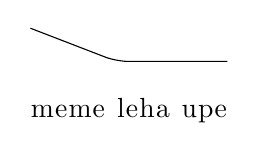
\begin{tikzpicture}
          \contour[contour raise=0.5cm]
          {|[6]meme |[2]leha upe|[2]}
        \end{tikzpicture}

        \begingl
        me\textasciitilde me[\textsc{erg\textasciitilde 1sg}]
        leha[have]
        upe[yam]
        \glft \transtext{Have some yams instead, eh?}
        \endgl
        \xe
        }
        \ex

        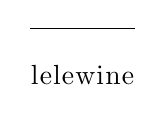
\begin{tikzpicture}
    \contour[contour raise=0.5cm]
    {|[2]lelewine|[2]}
  \end{tikzpicture}

  \begingl
  lelewine\textasciitilde\textasciitilde[\textsc{uncert}]
  \glft \transtext{Yams?}
  \endgl
  \xe
  \pagebreak
  {
    \color{red}
    \ex

    \begin{tikzpicture}
      \contour[contour raise=0.5cm]
      {|[2]wa |[5]luʔe |[3]kate|[2]}
    \end{tikzpicture}

    \begingl
    wa[\textsc{aff}]
    lu-ʔe[\textsc{obv-assoc}]
    kate[goodness]
    \glft \transtext{Yeah, good stuff.}
    \endgl
    \xe
    }
    \ex

    \begin{tikzpicture}
      \contour[contour raise=0.5cm]
      {|[4]luʔe kate\textasciitilde\textasciitilde|[2] |[7]atai leha tutu |[2]upe|[4]}
    \end{tikzpicture}

    \begingl
    kini-ʔe[\textsc{dem\_prox-assoc}]
    kate[goodness]
    atai[number\textsc{[q]}]
    leha[have]
    tu\textasciitilde tu[\textsc{erg\textasciitilde 2sg}]
    upe[yam]
    \glft \transtext{That's... alright. Yams--- how many do you have?}
    \endgl
    \xe
    {
      \color{red}
      \ex

      \begin{tikzpicture}
        \contour[contour raise=0.5cm]
        {|[2]me au|[4]ku\textasciitilde\textasciitilde|[2] |[2]ai|[4], |[2]ni|[4], |[2]ku,... |[6]niheu |[2]upe,|[1] |[4]ha kiniʔe|[2] |[5]kate|[2] |[5]pa ilaʔe |[4]xaku|[2]}
      \end{tikzpicture}

      \begingl
      me[\textsc{1sg}]
      auku[see]
      ai[one]
      ni[two]
      ku[three]
      niheu[ten]
      upe[yam]
      ha[four]
      kini-ʔe[\textsc{dem\_prox-assoc}]
      kate[goodness]
      pa[now]
      ilaʔe[gift\textsc{-assoc}]
      xaku[pain]
      \glft \transtext{I'll check... 1, 2, 3--- I’ve got ten, how’s four? A bit extra if it gets wild.}
      \endgl
      \xe}
      % With \nativetext{pa} rather than a more uncertain construction, the implication is that the happening is inevitable.

      \ex
      \begin{tikzpicture}
        \contour[contour raise=0.5cm]
        {|[2]wa|[2], |[4]kiniʔe kate|[2] - |[5]nataʔe kisuɸi|[3] ki|[1]}

      \end{tikzpicture}



      \begingl
      wa[\textsc{aff}]
      kini-ʔe[\textsc{dem\_prox-assoc}]
      kate[goodness]
      nata-ʔe[\textsc{dem\_med-assoc}]
      kisuɸi[\textsc{cert}]
      ki[big]
      \glft \transtext{Aye, this is nice -- that's a lot.}
      \endgl
      \xe

      {
        \color{red}
        \ex

        \begin{tikzpicture}
          \contour[contour raise=0.5cm]
          {|[2]wa suaki|[3] ɸai|[1] hipese|[3] pa upeʔe te|[1]le|[3]}

        \end{tikzpicture}


        \begingl
        wa[aff]
        suaki[wind\_blow]
        ɸai[\textsc{conj}]
        hipese[contain]
        pa[now]
        upe-ʔe[yam\textsc{-assoc}]
        tele[part]
        \glft \transtext{Hmm, since there’s a storm I’ll let you have them for less.}
        \endgl
        \xe
        }
        \ex

        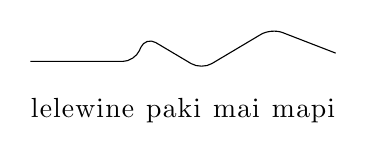
\begin{tikzpicture}
          \contour[contour raise=0.5cm]
          {|[2]lelewine|[2] |[5]paki|[1]  mai |[6]mapi|[3]}
        \end{tikzpicture}

        \begingl
        lelewine[\textsc{uncert}]
        paki[tell\_truth]
        mai[time]
        mapi[whole]
        \glft \transtext{If you insist, I'll always---}
        \endgl
        \xe

        {
          \color{red}
          \ex

          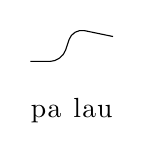
\begin{tikzpicture}
            \contour[contour raise=0.5cm]
            {|[2]pa|[2] |[6]lau|[5]}
          \end{tikzpicture}


          \begingl
          pa[now]
          lau[neaten]
          \glft \transtext{I'm gonna pack away soon, so just---}
          \endgl
          \xe
          }
          \ex

          
\begin{tikzpicture}
            \contour[contour raise=0.5cm]
            {|[4]wa|[6]}
          \end{tikzpicture}

          \begingl
          wa[\textsc{aff}]
          \glft \transtext{Yeah okay---}
          \endgl
          \xe
          {
            \color{red}
            \ex

            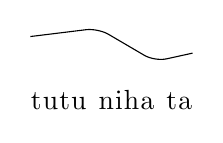
\begin{tikzpicture}
              \contour[contour raise=0.5cm]
              {|[4]tutu |[5]niha|[1] ta|[2]}
            \end{tikzpicture}

            \begingl
            tu\textasciitilde tu[\textsc{erg\textasciitilde 2sg}]
            niha[give]
            ta[\textsc{prox}]
            \glft \transtext{Just take them.}
            \endgl
            \xe
            }
            \ex

            \begin{tikzpicture}
              \contour[contour raise=0.5cm]
              {|[4]mapi|[4]ʔe |[2]ila|[3]}
            \end{tikzpicture}

            \begingl
            mapi-ʔe[whole\textsc{-assoc}]
            ila[gift]
            \glft \transtext{Free?}
            \endgl
            \xe
            {
              \color{red}
              \ex

              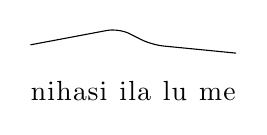
\begin{tikzpicture}
                \contour[contour raise=0.5cm]
                {|[2]nihasi |[4]ila|[2] lu me|[1]}
              \end{tikzpicture}


              \begingl
              niha-si[give\textsc{-inv}]
              ila[gift]
              lu[\textsc{obv}]
              me[\textsc{1sg}]
              \glft \transtext{You'll pay me later.}
              \endgl
              \xe}

              \ex

              \begin{tikzpicture}
                \contour[contour raise=0.5cm]
                {|[2]ɸawa|[1]si|[3]}
              \end{tikzpicture}


              \begingl
              ɸawa-si[thank\textsc{-inv}]
              \glft \transtext{Thank you!}
              \endgl
              \xe
              {
                \color{red}
                \ex

                \begin{tikzpicture}
                  \contour[contour raise=0.5cm]
                  {|[2]tu |[2]siʔe|[6]}
                \end{tikzpicture}

                \begingl
                tu[\textsc{2sg}]
                siʔe[brightness\textsc{-assoc}]
                \glft \transtext{Take care.}
                \endgl
                \xe
                }

                \ex

                \begin{tikzpicture}
                  \contour[contour raise=0.5cm]
                  {|[2]taʔe |[4]kate,|[2] |[5]iokusi|[3] a|[4]lete|[1] |[4]aukusi|[2]}
                \end{tikzpicture}

                \begingl
                ta-ʔe[\textsc{prox-assoc}]
                kate[good]
                i-auku-si[\textsc{pst.ipfv-}see\textsc{-inv}]
                alete[thus]
                auku-si[see\textsc{-inv}]
                \glft \transtext{Alright, see you later.}
                \endgl
                \xe


                {
                  \color{red}
                  \ex


                  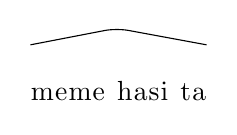
\begin{tikzpicture}
  \contour[contour raise=0.5cm]
  {|[2]meme |[4]hasi ta|[2]}
\end{tikzpicture}


\begingl
me\textasciitilde me[\textsc{erg\textasciitilde 1sg}]
hasi[continue]
ta[\textsc{prox}]
\glft \transtext{Goodbye.}
\endgl
\xe

\ex

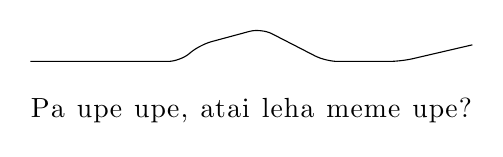
\begin{tikzpicture}
  \contour[contour raise=0.5cm]
  {|[2]Pa upe upe|[2], |[4]atai |[6]leha |[2]meme|[2] upe?|[4]}
\end{tikzpicture}

\begingl
pa[now]
upe[yam]
upe[yam]
atai[number]
leha[have\textsc{[q]}]
me\textasciitilde me[\textsc{erg\textasciitilde 1sg}]
upe[yam]
\glft \transtext{Yams, yams... shit, how many do I have left now?}
\endgl
\xe}
\end{comment}
\part{Translations}
\chapter{Smoyds}

\begin{subexamples}
  \ex
    \gloss
      fai & NEG \\
      'ike & know \\
      pane & person \\
      ana & near\_to \\
      me & 1SG \\
      'e & REL \\
      lu & OBV \\
      kamai & send \\
      ta & PROX \\
      wu & at \\
      ipe & house \\
      fa & POSS \\
      <me>me & <PL>1 \\
    \tr You do not know the friend that will come to our house.
  \ex
    \gloss
      fai & NEG \\
      'ike & know \\
      pane & person \\
      ana & near\_to \\
      me & 1SG \\
      'e & REL \\
      <me>me & <PL>1 \\
      ati'ihi & invite \\
      wu & at \\
      ipe & house \\
  \tr You do not know the friend we're inviting (here).
  \source 5moyd \#1330
\end{subexamples}

Both of these sentences describe the same event, however they are framed with opposing volition. In (a), the friend initiates, and in (b), the family does.

In both renditions, \transtext{friend} is rendered as \nativetext{pane ana me} \transtext{person near me}.

Familial bonds in particular are especially culturally significant for speakers of \langname . Coupled with the tendency for entire families to live together, and to only move out and part ways to start one's own family, the concept of closeness has extended into a linguistic metaphor for emotional attachment.

(a) uses the reflexive form of \nativetext{kamai}, emphasizing that this was done without prompting from the family (that is to say, this was previously unannounced and unknown). This contrasts with \nativetext{heemi} \transtext{to come}, which implies a relationship to the destination.

\nativetext{Lu} in (a) serves as a resumptive pronoun, allowing the reflexive reading of \nativetext{kamai ta}. This is necessary because \nativetext{pane ana me} is within a relative clause, and would otherwise leave \nativetext{ta} without a referent.

Also, \nativetext{wu} (in both cases) is being used to denote location, rather than performing its primary function conveying \transtext{on top}.

\begin{example}
  \gloss
    mai & time \\
    eta & age \\
    -'e & ASSOC \\
    pa & now \\
    pa\allo pami & ERG\allo marble \\
    ahi & fasten \\
    eusa & nose \\
  \tr When I was a child, I got a marble stuck in my nostril.
  \source 5moyd \#1289
\end{example}

\nativetext{Mai eta'e} must combine with the adverb \nativetext{pa} to form a topic-like adverbial phrase. This can be thought of as a phrase \nativetext{mai... pa} used to introduce a timeframe for the events following. Here, that frame is \nativetext{eta'e} \transtext{young age}, however this could be any number of things. One may expect a relative clause here, however, such a construction cannot be used for the purposes of temporal framing. Relative clauses are too syntactically heavy to fit this construction, and are generally \notabletext{determinate}.

One final note is that, as with other body parts, \nativetext{eusa} is left unmarked for possession when it is easily inferred (in most cases as the speaker when no other context is given).


\begin{example}
  \gloss
    <me>me & <ERG>1SG \\
    kisufi & CERT \\
    keke & eat \\
    neulina & stew \\
    tu'ase & wheat \\
    -la & ADJZ \\
    \tr I intend to eat oatmeal.
    \source 5moyd \#1252
  \end{example}

This is fairly standard, although the use of a certainty particle in place of \transtext{intend to} is more ambiguous than this translation makes it out to be. It could also be read as \transtext{I'll probably eat oatmeal.}, which could also be apt. In this situation, I've chosen to translate it as the first, meaning that we aren't sure whether some external factor will stop this from happening.

  \begin{example}
    \gloss
      <me>me & <ERG>1SG \\
      i- & PST.IPFV \\
      ka & open \\
      tepa & container \\
      pa & now \\
      siha & happen \\
      tele & part \\
      -la & ADJZ \\
    \tr I was opening the bottle and it shattered.
  \source 5moyd \#1228
\end{example}

Firstly, the choice to translate \transtext{bottle} with \nativetext{tepa} rather than a more specific word is because it is rare for drinking containers to be lidded, and so opening them wouldn't make sense.

In translating the verbs, it makes more sense to draw attention to the change of state of the bottle. Rather than implying the shattering is caused by the original agent (as using a particular verb for shattering would), the construction \nativetext{siha X-la} assumes that this happened on account of an external(/unintroduced) force, where \nativetext{-la} describes the end state. \nativetext{Pa} serves to link these clauses, and so rather than an unknown reading, we get a causative reading which is framed against the event rather than its original agent.

\begin{example}
  \gloss
    sulau & open \\
    tanu & door \\
    ta & PROX \\
    -'e & ASSOC \\
    kate & simplicity \\
  \tr The door opens easily.
  \alt To open this door is easy.
  \source 5moyd \#1395
\end{example}

The core argument of the verb phrase is deemphasized by being placed after the verb rather than before (as is typical with indicative phrases). This could also be interpreted as an interrogative, disambiguated solely through prosody. In very formal speech, deemphasized core arguments will be marked with the obviate, but this marking is usually unnecessary unless the deemphasis is particularly important or used to form contrast with another concept.

\nativetext{Ta} functions as a sort of topic marker, where \nativetext{kate} modifies the newly established topic. This strategy is common in forming simple adverbials.

\end{document}
